% Nome do capítulo
\chapter{Theoretical Foundation}
% Label para referenciar
\label{cap2}

% Diminuir espaçamento entre título e texto
\vspace{-1.9cm}

In this Chapter, we present concepts and techniques used throughout this work. We start
presenting smart cities, urban computing, and urban mobility concepts, and then,
information about how cities export their data 
on open data portals. Then, we show the GTFS
and its real-time extension, GTFS-RT,
which provides all the data required to execute our methodology.
Finally, we define the PTN as a complex network after 
a gentle introduction to complex networks and graphs.

\section{Smart Cities}
There are many definitions of smart cities, \citeonline{pardo2011} describe
a smart city is a city whose "data infuses information into its physical infrastructure to improve
conveniences, facilitate mobility, add efficiencies, conserve energy,
improve the quality of air and water, identify problems, and fix them
quickly, recover rapidly from disasters, and collect data to make better
decisions, deploy resources effectively, and share data to enable
collaboration across entities and domains".

In addition, a smart city must be connected to its citizens and 
various systems, for instance, transportation, health care, and more.
The dimensions of a smart city are its networked infrastructure enabling
political efficiency and social and cultural development. It is social inclusion
and social capital in urban development. Another key point %estranho
is the measurement of performance indexes, which help keep the focus 
on resources and time where they are needed \cite{smart_cities_SLR}. Finally, it is worth highlighting that the assessment of a smart city must be adapted to each 
specific scenario to develop the quality of life of its citizens.

\subsection{Urban Computing}
Urban computing is an interdisciplinary toolkit that uses the data generated by the sources in 
urban spaces to tackle the major issues that cities face \cite{urban_computing}. 
This toolkit comprises processes of acquisition, integration, and analysis of the data
generated, which sources could be sensors, devices, vehicles, buildings, and humans,
for instance. The problems faced are also interdisciplinary, they could be related to
many fields, such as 
transportation \cite{Silveira2015, 10.1145/3394486.3412856, GTFS-RT_delays_2017, GTFS-RT_delays_2022, routableTimetableGTFS, GTFS-RT_delays_2022-ADWIN}, 
and health \cite{Ro2020, Saran2020, Chang2020, Sonkin2020}.



\subsection{Human mobility}
Human mobility aims to study the movement of humans through time and space. And its
impacts on the environment, understanding human mobility benefits many study fields,
such as traffic forecasting \cite{GTFS-RT_delays_2022-ADWIN},
urban planning, 
and tourism \cite{Carvalho2018}. 
Before introducing techniques and methods using urban computing, it is
fundamental to briefly introduce its history, which dates
back to the 19th century with the {\em Laws of Migration} \cite{lawsofmigration}.
These laws try to explain predictions of migration patterns using 
socio-economic factors, despite the observational character, they are non-quantitative.
Later on in the 1940s, \citeonline{lawofinterveningopportunities} introduced the 
{\em Law of Intervening Opportunities} that \citeonline{human_mobility_SLR} defines
as "the number of people going a given distance is directly proportional to
the number of opportunities at that distance and inversely to the number of
intervening opportunities." In other words, when migrating, the further you are
willing to displace, the more opportunities you should have. However, unexpected 
suitable opportunities may appear before the person arrives at the original destination,
called intervening opportunities.

\citeonline{zipf1941national} applied his law from observing the rank-frequency dependence in linguistics, the eponymous Zipf's law.
This infers that the frequency of a word ranked $z$ has the statistical dependence
of $f_z \sim 1/z$, in terms of usage \cite{human_mobility_SLR}. When Zipf applied
this law to cities, the rank $z$ was not a constant yet varied due to two competing
forces: Diversification and unification. The first expresses
the likelihood of the population living near the source of raw materials to 
shorten the distances to the production center, leading to multiple centers of a small population. 
The second force describes the inclination of populations to concentrate in urban centers
causing the minimization of work required to transport finished products to consumers,
leading to a large population in few centers.

In the 1990s, human mobility methods allowed to model more complex human
dynamics by incorporating a space-time prism using \ac{GIS} techniques
\cite{spacetime1991}. So, the models used spatial and temporal
constraints upon an individual's movement patterns to enrich the analysis.
Yet, in the 1990s, despite upgrading the models, the data available failed to
calibrate the models, which issue was solved in the 21st century
\cite{human_mobility_SLR}. GPS data usage became well-adopted with
mobile phones, and this scenario led to the development of 
more complex data mining methods. 

Also, in the 21st century, we live \citeonline{zipf1941national}'s scenario
of few centers with large populations, but along with urban computing methods 
from this century led to the improvement of mobility methods in the urban space
to a level of real-time services to mass populations. These models 
are based on the premise that every day, many citizens are going to
displace over the whole city, this could be done in many ways, such as 
walking, cycling, driving, and using public transportation. Consequently, these models help cities make decisions considering their own data.
Thus, understanding the patterns underneath and their history is the key point to create effective models, such as
identifying delays and other public transportation questions.



\section{GTFS and GTFS‑RT specifications}

\subsection{GTFS}
The General Transit Feed Specification defines a common format for
public transportation schedules and associated geographic information \cite{GTFS}.
Google has defined publish patterns for public transit agencies to improve collaborative work between public transit agencies and 
developers. This standardization helps developers design applications that consume that data interoperable \cite{GTFSpioneering}. 


This specification comprises {\em feeds}, a series of text files collected
in a ZIP file. This set of files of a feed is called {\em dataset}, and each file in a 
dataset corresponds to an {\em entity} from the Figure \ref{img:2:1} \cite{wong2013}. A {\em record}  represents a single entity, a data structure comprised of several different field values, represented in a table as a row. A {\em field} of one record represents a property
of this entity, represented in a table, as a column. Neither all files from the dataset nor
all fields of one record are required, GTFS has three kinds of {\em field values}:
\begin{enumerate*}
    \item {\em Required}, the field must be included in the dataset, and a value must be provided in that field for each record.
    \item {\em Optional}, the field may be omitted from the dataset.
    \item {\em Conditionally required}, the field or file is required under certain conditions outlined in the field or file description. Outside of these conditions, this field or file is optional
\end{enumerate*}
\cite{GTFS}.

The GTFS has been studied in many research fields. The specification provides
the Collective Transportation Network that is used to model a multimodel urban
transportation network, which is a network that has at least two modes. The user
has to transfer between modes \cite{gtfsexemple3}. The multimodel urban 
transportation network can be understood as the composition of the street network
and the infrastructure for each modal, bus and train, for instance. Furthermore,
GTFS is also used for ridesharing or carpooling applications where 
users share a private vehicle to make the same or similar trip \cite{GTFSExemples}.


\begin{figure}[t]
     \centering
        \caption{GTFS data structure}
        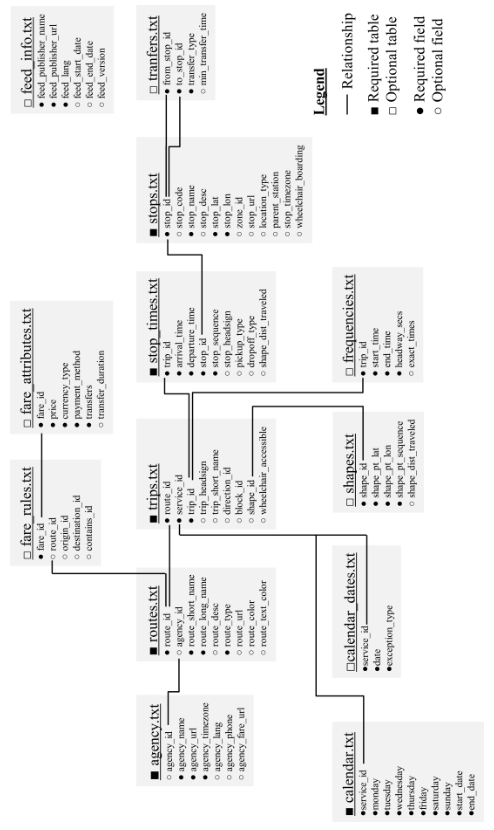
\includegraphics[scale=0.50, angle=270]{imagem/cap2/gtfs_wong.png}
        \source{\citeonline{wong2013}}
        \label{img:2:1}
    \end{figure}
\subsection{GTFS-RT}
On the one hand, the GTFS provides static data of schedules, maps, and fares, on the other hand, 
it neither supplies vehicle positions nor trip updates nor service alerts, natively. The GTFS-RT
is an extension of GTFS, allowing public transportation agencies to provide 
real-time updates about their fleet. Currently,
it supports three types of information served via HTTP and is updated
frequently. Its transmission is based on regular binary files, and there are no 
constraints on how frequently the feed should be updated or retrieved \cite{GTFS-RT}.
The types are listed as:
\begin{itemize}
  \item \textbf{Trip updates} - delays, cancellations, changed routes.
  \item \textbf{Service alerts} - stop moved, unforeseen events affecting a station, route, or the entire network
  \item \textbf{Vehicle positions} - information about the vehicles, including location and congestion level
\end{itemize}

The delays worsen the user experience with the PTN,
GTFS-RT has enabled many researchers to estimate, analyze, and mitigate delays,
due to the temporal features available.
One approach is to stream significant delay changes in
real-time \cite{GTFS-RT_delays_2022-ADWIN}, 
in other words, the user can be notified in real-time with 
schedule deviation. Another approach to mitigate delays is
to collect real-time data and use the temporal series to
predict delays and improve the timetable
\cite{GTFS-RT_delays_2017, GTFS-RT_delays_2022}.

GTFS and GTFS-RT specifications are important in many research fields, such as human mobility. 
Then, it is necessary to comprehend these two specifications to develop a framework to fulfill the GTFS-RT, which could be unavailable, with real-time data from an API combined with GTFS. Finally, our approach uses data structures alike GTFS-RT, as further discussed in Chapter \ref{cap4}.


\section{Complex Networks and Graphs}
In the late 1990s and early 2000s, computational models started to 
deal with huge datasets, which have been only increasing since then. 
In this scenario, complex networks appear to address this issue
based on graph theory designed to model real-world networks, and these models
are suitable to represent relationships and interactions 
between entities through link orientation and labels \cite{barabasiCN}.
Complex networks present compact structures, also called {\em small worlds},
with short distances between nodes, high levels of correlations, and self-organization
\cite{ferber2012}.
The popularization World-Wide Web and its applications, chemistry, drug 
design, natural language processing, and recommender
systems are examples of applications in which complex networks could be used.
To understand a complex network and its metrics, we need to comprehend 
some graphs concepts.

\citeonline{Bacciu_2020} state that "a graph has a compositional nature, being 
a compound of atomic information pieces and a relational nature, as the links
defining its structure denote relationships between the linked entities".
To formally define a graph, the mathematical notation is  \textit{$g = (V_g, E_g, X_g, A_g)$}
where $V_g$ a set of {\em vertexes} and $E_g$ is a set of {\em edges}, or {\em arcs} 
connecting a couple of nodes \cite{graph}. Two more sets, $X_g$ and $A_g$, represent additional information on the node set and the edges set, respectively. In other words, the nodes and edges in some applications have extra features. So, each node $u \in |V_g|$
has a unique feature vector associated therefore, each edge is associated with 
and feature vector $a_{uv} \in A_g$. 

When couples of nodes are ordered, i.e., 
$E_g \subseteq \{\{u,v \} | u,v \in V_g\}$, in a graph, this graph is {\em directed} and its 
edges are {\em oriented}, otherwise the graph is {\em undirected} and its edges 
are {\em non-oriented}. In both directed and undirected graphs, a {\em walk} is a sequence of 
edges that join a sequence of vertexes, a {\em trail} is a walk in which all edges are distinct,
and a {\em path} is a trail in which all nodes are distinct
\cite{williamsonlists}.

\subsection{Public Transportation Networks as a complex network}

The public transportation network is one of the networks that is 
part of the lives of millions of people around the globe, but it 
hides a high complexity degree \cite{ferber2012}.
The PTN can be represented as a {\em directed} graph $G=(V_g,E_g,X_g,A_g)$,
where the set of nodes $V_g$ represents the bus stops and
the set $E_g$ represents the directed arcs that connect different bus stops.
$X_g$ and $A_g$ are the sets of additional information about the nodes 
($V_g$) and the arcs ($E_g$), respectively. Figure \ref{img:2:2} shows $G$. 

    \begin{figure}[H]
     \centering
        \caption{The PTN modeled as the graph $G$}
        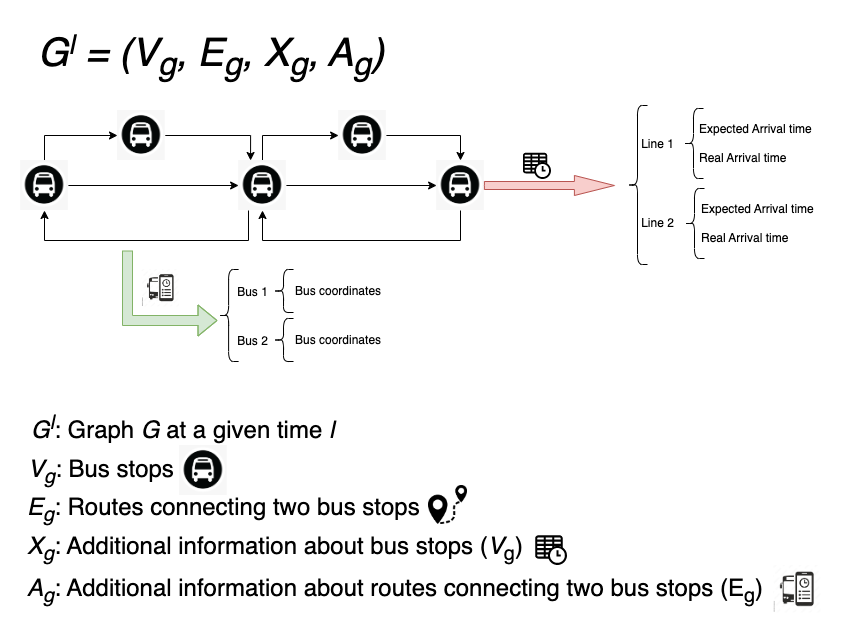
\includegraphics[scale=0.5]{imagem/cap2/final_graph.png}
        \source{The authors}
        \label{img:2:2}
    \end{figure}

$X_g$ contains the bus arrival time on each bus stop in $V_g$. Which is
comprehended as all bus trips that pass by any bus stop $v$ in $V_g$
during a day, for instance. And,
$A_g$ contains the bus entries collected between two sequenced bus stops, $B_x$ and 
$B_{x+1}$. In other words, that is all the information provided by a bus while
traveling through any arc $e$ of $E_g$.


The graph $G$ is a {\em dynamic} graph because the routes change over the days, so the structure of this graph is not fixed.
But, when we approach this graph in a defined time interval, it has a {\em static} topology because the bus stop locations and routes
are not on the same day. Thus, this graph can be
modeled using two data groups, static data, and RT data.
The first group is represented by the GTFS data which is used to generate $V_g$ and
$E_g$ sets, since both sets do not change over the delimited time interval. The second group of data is represented by the real-time bus entries producing $X_g$ and $A_g$ sets, which change over the delimited time interval, meaning
that the traffic will be different on Monday than Tuesday, for example. 

